% Preamble
%
\documentclass[a4paper,09pt]{article}

\usepackage[familydefault,light]{Chivo}
\usepackage{stmaryrd}
\usepackage[utf8]{inputenc}
\usepackage{xcolor}
\usepackage[pdftex]{graphicx}
\usepackage[english]{babel}
\usepackage{float}
\usepackage{hyperref}
\hypersetup{colorlinks=true,linkcolor=magenta}

%% Tikz
\usepackage{tikz}
\usetikzlibrary{arrows}

% to set size for itemize in node
\usepackage{varwidth}

% to reduce left margin of itemize
\usepackage{enumitem}
\setlist{leftmargin=0mm}

\tikzset{
  class/.style={
    rectangle,
    rounded corners,
    draw=black, very thick,
    minimum height=2em,
    inner sep=4pt,
    text centered,
  },
}

% use for the 'parser'
\usepackage{etoolbox}

% second try of foreach loop
\newcommand\handler[1]{\item[-] #1}
\DeclareListParser*\forsemicolonlist{;}

% provides \isempty test
\usepackage{xifthen}

\usepackage{enumitem}
% \newclass{class name}{attribute <list>}{method <list>}
% attribute list and method list are list with ',' as separator
\newcommand{\newclass}[3]{
  {
    \begin{tabular}{l}
     \renewcommand{\arraystretch}{1.5}
      \large{\textbf{#1}}
      \ifthenelse{\isempty{#2}}{}{
      \\
      \hline
      \textbf{Attribute}\\
      {\begin{varwidth}{\linewidth}\begin{itemize}[noitemsep]
            \forsemicolonlist\handler{#2}
          \end{itemize}\end{varwidth}}
      }
      \ifthenelse{\isempty{#3}}{}{
      \\
      \hline
      \textbf{Method}\\
      {\begin{varwidth}{\linewidth}\begin{itemize}[noitemsep]
            \forsemicolonlist\handler{#3}
          \end{itemize}\end{varwidth}}
      }
   \end{tabular}}
}

\newcommand{\newtable}[2]{
  {
    \begin{tabular}{l}
     \renewcommand{\arraystretch}{1.5}
      \large{\textbf{#1}}
      \ifthenelse{\isempty{#2}}{}{
      \\
      \hline
      {\begin{varwidth}{\linewidth}\begin{itemize}[noitemsep]
            \forsemicolonlist\handler{#2}
          \end{itemize}\end{varwidth}}
      }
   \end{tabular}}
}

\usepackage{lscape}
\usepackage{rotating}

%% Scala colours
\newcommand{\trait}[1]{\textcolor[rgb]{0.8,0,0}{$\mathsf{<\!trait\!>}$} #1}
\newcommand{\type}[1]{\textcolor[rgb]{0.8,0.4,0}{$\mathsf{#1}$}}
\newcommand{\method}[1]{\textcolor[rgb]{0.2,0.4,0.4}{$\mathsf{#1}\ $}}
\newcommand{\attribut}[1]{\textcolor[rgb]{0,0.8,0.2}{$\mathsf{#1}\ $}}  


% Commands
%
%% So we can highlight things (YBG is for Yellow BackGround, if you want to
%% create new ones - power to the colours ! - follow the convention ;)

\newcommand{\YBG}[1]{\colorbox[rgb]{1,1,0.3}{#1}}

% Document
%

\setlength{\parindent}{0cm}

\author{Elie Canonici Merle, Colin González, Sylvain Ribstein, \\
  Kevin Sanchis, Anas Aarab, Paul Laforgue}

\title{Architecture and Design}

\date{October 24, 2016 \\ \small Last updated : \today}

\begin{document}

\maketitle

\begin{abstract}
  This file provides an the software architecture of the project of the
  course POCA 2016.
\end{abstract}

\tableofcontents

\section*{Introduction}

\textbf{KEYWORD}:
\textit{scalability, separation of concerns, quality-driven, reusable solutions}.

We are focused on:

\begin{itemize}
\item \textbf{Liveness}: the operations eventually return something.
\item \textbf{Safety}: the operations never return anything incorrect.
\end{itemize}

% \section{Concept}
+++
% \begin{sidewaysfigure}
%   \include{example_diagram}
% \end{sidewaysfigure}

\section{Architecture Description}

\subsection{Core}
The core of the architecture holds within itself the most important features. In order to provide a correct program we try to keep the core as abstract as possible. One very important goal of the core is to give a framework capable to handle concurrency while respecting the properties of liveness and safety. However, having massive players implies a challenge in order to prevent lostupdates and keep some coherence. The strategy is to simulate Lamport's one writer, $n$ readers regular multivalued register. Where the data is stored in shared memory, here a database. To keep clients updated, we shall use timestamps that validate or invalidate data. One advantage of using a register like model is that it has been verified and proved a robust and reliable model in concurrent applications. In the UML figure \ref{coreuml} we see the relationship between each object and its caracteristics.\\
\subsection{BUS}
The bus is a trivial abstraction of the communication bus, most likely a WAN TCP connection. However, since implementation hasn't been fixed, we prefer using an abstraction in the architecture giving the ability to other implementations further.
\subsection{Abstract Server}
We have chosen to admit that the engine, the database interface appilcation and  the clients are treated as servers. This enables a horizontal model of extensability and no hierarchy between this objects respecting the philosophy of Scala. On the other hand, having non hierarchical objects makes it difficult to understand which program is playing a keyrole for an attacker giving more security. Servers are expected to implement the methods of the Serverizable interface. In fact, a client program is not always ran in server mode. Servers communicate with each other through BUS objects. In some cases, abstract servers might have to accept several connections. A server accepting connections are called $hosts$ and servers connecting to other servers $guests$.

\subsection{Token}
Pokemon like tokens, points of interests and possibly other users are represented as tokens to the client. This tokens are instancieted at run time with data stored in de database.

\subsection{TokenCollection}
Tokens are expected to be used as collections. The class TokenCollection provides this feature. This way, it is easy to manage several tokens at a time.

\subsection{Interaction between abstract servers}
In order to implement the  model of the register, the write operations are done by the engine object and read operations by the engine and clients objects. The engine, allows to bufferise client's write requests , and write \"atomically\" to the database. The database, represents the shared memory here of the register.

\begin{sidewaysfigure}
  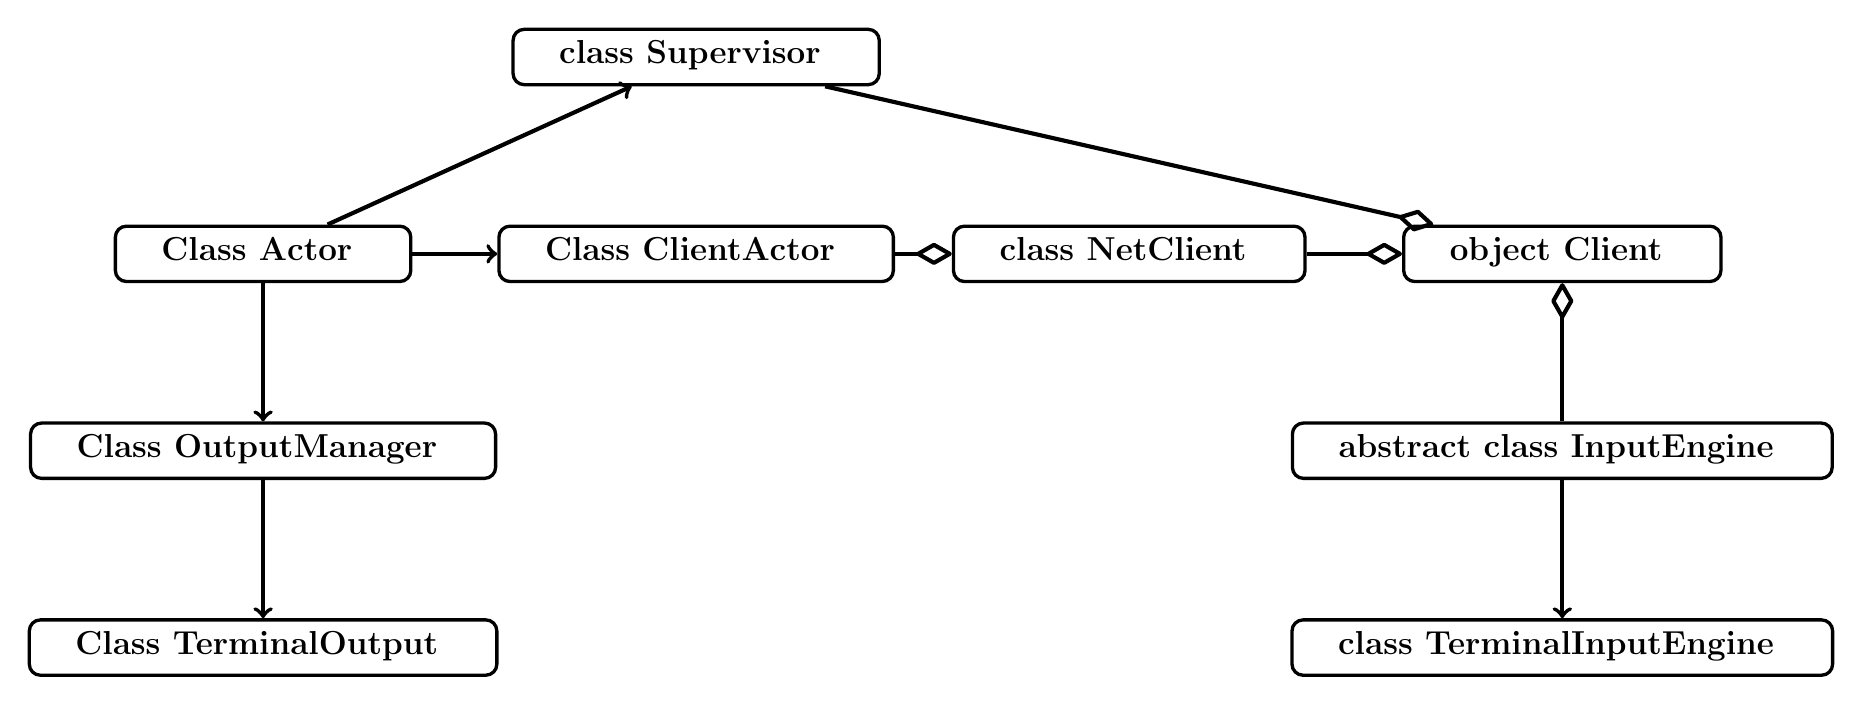
\begin{tikzpicture}
    % \node[class] (InputMsg){
    % \newclass{Object InputMsg} {
    % \attribut{case class Login}(\type{string},\type{string});
    % \attribut{case class Signup}(\type{string},\type{string});
    % ...} {}};

    % \node[class] (OutputMsg){
    % \newclass{Object OutputMsg} {
    % \attribut{case class InfoText}(\type{string});
    % \attribut{case class Pokemons}(\type{Seq[Pokemon]});
    % ...} {}};

    \node[class] (TerminalOutput) {
      \newclass{Class TerminalOutput}{}
      {}
    };

    \node[class] (OutputManager) [above of=TerminalOutput, node distance=2.5cm] {
      \newclass{Class OutputManager} {}
      {
        % \method{display}(\type{String}) : \type{Future[Unit]};
        % \method{displays}(\type{Seq[String]}) : \type{Future[Seq[Unit]]};
        % \method{output}(\type{Msg}):\type{Reiceve};
      }
    };

    \node[class] (Actor) [above of=OutputManager, node distance=2.5cm] {
      \newclass{Class Actor} {}
      {}
    };

    \node[class] (ClientActor) [right of=Actor, node distance=5.5cm] {
      \newclass{Class ClientActor} {}
      {}
    };

    \node[class] (NetClient) [right of=ClientActor, node distance=5.5cm] {
      \newclass{class NetClient} {}
      {
        % \method{apply}:\type{NetClient}
      }
    };

    \node[class] (Supervisor) [above of=ClientActor, node distance=2.5cm] {
      \newclass{class Supervisor} {
        % \attribut{val output} : \type{Actor}
      }
      {
        % \method{whenloggedout} : \type{Receive};
        % \method{whenloggedin} : \type{Receive}
      }
    };

    \node[class] (Client) [right of=NetClient, node distance=5.5cm] {
      \newclass{object Client} {
        % val net : \type{NetClient};
        % type type{I}<:\type{InputEngine};
        % val system : \type{Actor};
        % val supervisor : \type{Actor};
        % val inputEngine : \type{I};
      }
      {
        % \method{run}:\type{unit}
      }
    };

    \node[class] (InputEngine) [below of=Client, node distance=2.5cm] {
      \newclass{abstract class InputEngine} {}
      {
        % \method{run}:\type{Future[Any]}
      }
    };

    \node[class] (TerminalInputEngine) [below of=InputEngine, node distance=2.5cm] {
      \newclass{class TerminalInputEngine} {}
      {
        % \method{run}:\type{Future[unit]};
        % \method{read}:\type{unit}
      }
    };

    \path
    (OutputManager) edge [->,line width=1.5pt] node {} (TerminalOutput)
    (Actor) edge [->,line width=1.5pt] node {} (OutputManager)
    (Actor) edge [->,line width=1.5pt] node {} (Supervisor)
    (Actor) edge [->,line width=1.5pt] node {} (ClientActor)
    (InputEngine) edge [->,line width=1.5pt] node {} (TerminalInputEngine)

    (Supervisor) edge [-open diamond, line width=1.5pt] node {} (Client)
    (NetClient) edge [-open diamond, line width=1.5pt] node {} (Client)
    (ClientActor) edge [-open diamond, line width=1.5pt] node {} (NetClient)
    (InputEngine) edge [-open diamond, line width=1.5pt] node {} (Client)
    ;  

  \end{tikzpicture}
  \caption{UML of the Client}
  \label{clientuml}
\end{sidewaysfigure}

\begin{sidewaysfigure}
  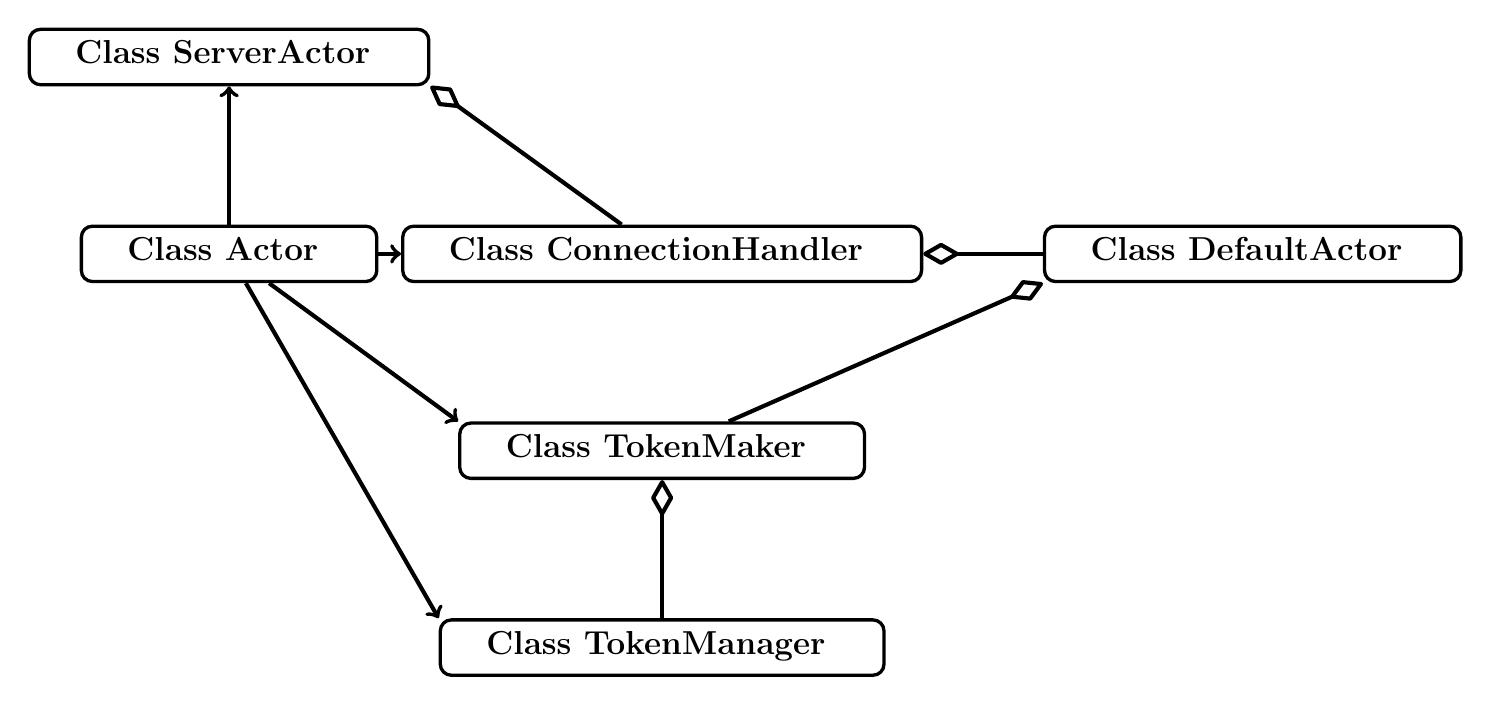
\begin{tikzpicture}

    \node[class] (ServerActor) {
      \newclass{Class ServerActor} {}
      {}
    };

    \node[class] (Actor) [below of=ServerActor, node distance=2.5cm] {
      \newclass{Class Actor} {}
      {}
    };

    \node[class] (CH) [right of=Actor, node distance=5.5cm] {
      \newclass{Class ConnectionHandler} {}
      {}
    };

    \node[class] (DefaultActor) [right of = CH, node distance=7.5cm] {
      \newclass{Class DefaultActor} {}
      {}
    };

    \node[class] (TokenMaker) [below of= CH, node distance=2.5cm] {
      \newclass{Class TokenMaker} {}
      {}
    };

    \node[class] (TokenManager) [below of= TokenMaker, node distance=2.5cm] {
      \newclass{Class TokenManager} {}
      {}
    };

    \path
    (Actor) edge [->,line width=1.5pt] node {} (ServerActor)
    (Actor) edge [->,line width=1.5pt] node {} (CH)
    (Actor) edge [->,line width=1.5pt] node {} (TokenMaker.north west)
    (Actor) edge [->,line width=1.5pt] node {} (TokenManager.north west)

    (TokenMaker) edge [-open diamond, line width=1.5pt] node {}
    (DefaultActor.south west)
    (TokenManager) edge [-open diamond, line width=1.5pt] node {} (TokenMaker)
    (DefaultActor) edge [-open diamond, line width=1.5pt] node {} (CH)
    (CH) edge [-open diamond, line width=1.5pt] node {}
    (ServerActor.south east) 
    ;  
    
  \end{tikzpicture}
  \caption{UML of the Server}
  \label{serveruml}
\end{sidewaysfigure}
\begin{sidewaysfigure}
  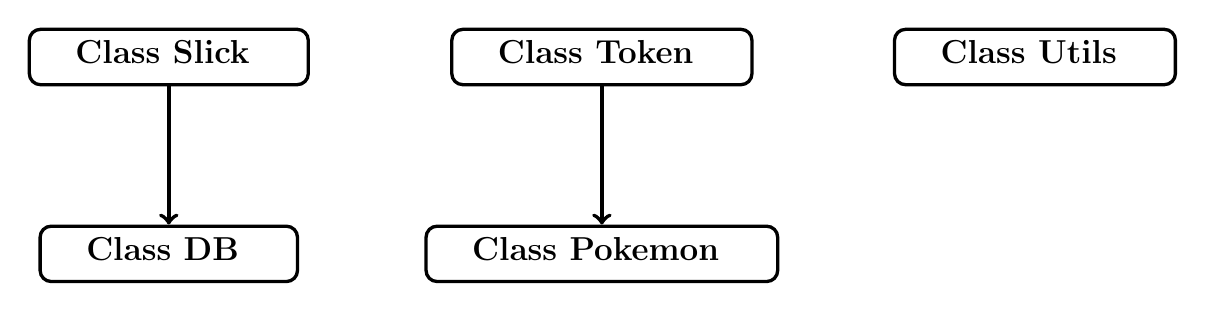
\begin{tikzpicture}

    \node[class] (Slick)  {
      \newclass{Class Slick} {}
      {}
    };

    \node[class] (DB) [below of=Slick , node distance=2.5cm] {
      \newclass{Class DB} {}
      {}
    };

    \node[class] (Token) [right of=Slick , node distance=5.5cm] {
      \newclass{Class Token} {}
      {}
    };

    \node[class] (Pokemon) [below of=Token , node distance=2.5cm] {
      \newclass{Class Pokemon} {}
      {}
    };

    \node[class] (Utils) [right of=Token , node distance=5.5cm] {
      \newclass{Class Utils} {}
      {}
    };

    \path 
    (Token) edge [->,line width=1.5pt] node {} (Pokemon)
    (Slick) edge [->,line width=1.5pt] node {} (DB)

    ;
  \end{tikzpicture}
  \caption{Other Class}
  \label{otheruml}
\end{sidewaysfigure}



% \begin{tikzpicture}
   
%   \node[class] (BUS) {
%     \newclass{Class BUS}
%     {
%     }{
%       \method{this}(UID: \type{int},pass:\type{string}):\type{Boolean};
%       \method{Send}(req:\type{request}):\type{Boolean} ;
%       \method{Receive}():\type{Result} ;
%       \method{Disconnect}(): \type{Boolean}
%     }
%   };
  
%   \node[class] (TCP) [below of=BUS, node distance=2.5cm,xshift=1cm] {
%     \newclass{Bus}
%     {}{}
%   };
  
%   \node[class] (HTCP) [below of=TCP, node distance=1cm] {
%     \newclass{HostBus}
%     {}{}
%   };

%   \node[class] (HBUS) [below of = BUS, node distance = 7cm]{
%     \newclass{Class HostBUS}
%     {
%       \attribut{Port}:\type{Int};      
%     }
%     {
%       \method{this}():();
%       \method{Accept}(UID:\type{Int},pass:\type{String}):();
%       \method{send}(req:\type{request}):\type{Boolean} ;
%       \method{Receive}():\type{Result} ;
%       \method{Disconnect}():();
%     }
%   };

%   \node[class] (OBJ) [right of=BUS, node distance=7cm] {
%     \newclass{Abstract Server}
%     {
%       \attribut{UID}:\type{Int};
%       \attribut{Address}:\type{IP};
%       \attribut{Port}:\type{Int};
%       \attribut{Timeout}:\type{Int};
%       \attribut{Maxconnection}:\type{Int}
%     }{
%     }
%   };

%   \node[class] (SRV) [right of=OBJ, node distance = 8cm] {
%     \newclass{Engine}
%     {
%       \attribut{CltBus}: \type{HostBUS};
%       \attribut{SrvDBBus}: \type{BUS}
%     }{
%       \method{setToken}(tok:\type{Token}):\type{Boolean};
%       \method{getToken}(req:\type{Request})\type{Token}
%     }
%   };
  
%   \node[class] (SDB) [below of=SRV, node distance=5cm] {
%     \newclass{DB Server}{
%       \attribut{DB\_IP}:\type{IP};
%       \attribut{DB\_port}:\type{Int};
%       \attribut{DB\_connect}:\type{Socket};
%       \attribut{Bus}:\type{HostBUS};
%     }{
%       \method{connectDB}():\type{Boolean};
%       \method{requestDB}(q:\type{Query}):\type{Result}
%     }
%   };

%   \node[class] (CLT) [below of=SDB, node distance =6cm] {
%     \newclass{Client}
%     {
%       \attribut{UserID}:\type{Int};
%       \attribut{Poke}: \type{Token\ Collection};
%       \attribut{POI} : \type{Token\ Collection};
%       \attribut{PokeArea}: \type{Token\ Collection};
%       \attribut{POIArea}: \type{Token\ Collection};
%       \attribut{SrvDBBus}: \type{BUS};
%       \attribut{SrvBus}: \type{BUS};
%       \attribut{CltBus}: \type{HostBUS\ option}
%     }{
%       \method{connect}(user:\type{String},pass:\type{String}):(UserID:\type{Int});
%       \method{getToken}(req:\type{Request}):\type{Token};
%       \method{setToken}(tok:\type{Token}):\type{Boolean};
%       \method{getAllToken}(req:\type{Request}):\type{Token\ Collection};
%       \method{areaToken}(coord:\type{GPS},req:\type{Request}):\type{Token\ Collection}
%     }
%   };

%   % \node[class] (SRVI) [right of=SDB, node distance =8cm] {
%   %   \newclass{Trait Serverizable}
%   %   {
%   %     \attribut{Timeout}:\type{Int};
%   %     \attribut{Maxconnection}:\type{Int};
%   %   }{
%   %     \method{CreateBus}(port:\type{Int}):();
%   %     \method{Accept}(UID:\type{Int},passphrase:\type{String}):();
%   %     \method{Disconnect}():();
%   %   }
%   % };

%   \node[class] (TCL) [left of=CLT, node distance = 8cm] {
%     \newclass{Token collection}
%     {
%       \attribut{Token}:\type{HashTable}
%     }{
%       \method{del}(tok:\type{Token}):();
%       \method{add}(tok:\type{Token}):();
%       \method{hash}():()
%     }
%   };

%   \node[class] (TOK) [left of=TCL, node distance=5cm] {
%     \newclass{Token}{
%       \attribut{DBID}:\type{Int}
%     }{
%     }
%   };

%   \node[class] (POK) [below of=TOK, node distance=2.8cm,xshift=-2.5cm]{
%     \newclass{Pokemon}
%     {
%       \attribut{Name}:\type{String};
%       ...
%     }{
%     }
%   };

%   \node[class] (POI) [below of=TOK, node distance=2.8cm,xshift=2.5cm]{
%     \newclass{Point of Interest}
%     {
%       \attribut{Name}:\type{String};
%       ...
%     }{
%     }
%   };

%   \path
%   (TCP) edge [->,line width=1.5pt] node {} (BUS)
%   (HTCP) edge [->,line width=1.5pt] node {} (HBUS)
%   (OBJ) edge [-open diamond, line width=1.5pt] node {} (TCP.north east)
%   (OBJ) edge [-open diamond, line width=1.5pt] node {} (HTCP.north east)
%   (SRV) edge [->, line width=1.5pt] node {} (OBJ)
%   (CLT.north west) edge [->, line width=1.5pt] node {} (OBJ)
%   (SDB.north west) edge [->, line width=1.5pt] node {} (OBJ)
%   % (SRV) edge [loosely dashed,->, line width=1.5pt] node {} (SRVI)
%   % (CLT.north east) edge [loosely dashed,->, line width=1.5pt] node {} (SRVI)
%   % (SDB) edge [loosely dashed,->, line width=1.5pt] node {} (SRVI)
%   (TCL) edge [-open diamond, line width=1.5pt] node {} (TOK)
%   (POK) edge [->,line width=1.5pt] node {} (TOK)
%   (POI) edge [->,line width=1.5pt] node {} (TOK)
%   (CLT) edge [-open diamond, line width=1.5pt] node {} (TCL);
  
% \end{tikzpicture}




\subsection{Protocol}


\subsubsection{Technical specification}

\textbf{Player}

\begin{itemize}
\item In order to play, the player must sign in.
\item He gives his username and password, the server will ask the database and
  send him a message which can be a connection to the game (the server will
  then load the last known state of the player : items, pokémons, position...)
  or a denial.
\item If the player doesn't exist in the database, he has to create an account.
  He can do so by providing an username and a password to the server.
\item While in-game, The player can do many actions :\\
- Move to a location in the map with x,y coordinates or via GPS position.\\
- List his items.\\
- List his collection of pokémons.\\
- Interact with tokens (point of interest, pokémons or other players).\\
\end{itemize}

\textbf{Server}
\begin{itemize}
\item Receives messages from player and send queries to the database.
\item Sends information or acknowledgement to a player.\\
\end{itemize}

\textbf{Actions in details}
\begin{itemize}
\item The client/player wants to move to a location x,y. He asks the server.
  The server will update his position in the database, and will update the
  map. He will then send an acknowledgement to the client.
\item The client/player signs in. The server will check if the username and
  the password exists in the database. If so, the player will be able to play,
  if not, he can retry or create an account.
\item The client/player wants to see his items/pokémons. He asks the server.
  The server will get the list of items/pokémons in the database and send it
  to him. The client will send an acknowledgement to the server.
\item If the client/player interacts with a token, this will be notified to
  the server and will have consequences :\\
  - If he interacts with a POI, he can get items from it. (and the server will
  update his items).\\
  - If he interacts with a pokémon, he can catch it (and the server
  will update his collection).\\
- If he interacts with a player...\\
\end{itemize}

\subsubsection{Functional specification}

These messages can be sent to the server by the client or to a client by the server :

\begin{itemize}
\item \textbf{SIGNusername:password} : The client signs in with username and password.
\item \textbf{SIOK} : The server informs the client that he's connected to the game.
\item \textbf{SINO} : The server informs the client that his account doesn't exist.
\item \textbf{CACCusername:password} : The client wants to create an account.
\item \textbf{CAOK} : The server informs the client that his account is created.
\item \textbf{CANO} : The server informs the client that his account creation
  failed (already exists in the database).\\
\item \textbf{GETI} : The client wants to see his items.
\item \textbf{ITEM[items]} : The server sends a list of item to a player/client.
\item \textbf{ITOK} : The client sends an acknowledgement to the server when he
  receives the list of item.
\item \textbf{GETC} : The client wants to see his collection of pokémons.
\item \textbf{COLL[pokemons]} : The server sends a list of Pokémons to a player/client.
\item \textbf{COOK} : The client sends an acknowledgement to the server when he
  receives the list of pokémons.
\item \textbf{MOVEx:y} : The clients wants to move to a location (x,y).
\item \textbf{MOOK} : The server updates the player's position in the
  database, and the map.\\
\item \textbf{IWPOIpoi} : The client wants to interact with the POI 'poi'.
\item \textbf{POID} : The server updates the state of the player (his list of items)
  and the state of the POI (has been visited by this player).
\item \textbf{IWPOKpokemon} : The client wants to interact with the 'pokemon'.
\item \textbf{POKD} : After the mini-game, the server updates the state of the player
  (his list of pokémons and items).
\end{itemize}

\subsection{Database model}


The diagram for \textit{Connection and data acceses} is presented in figure
\ref{ConnDataAccess}.
We are using the modern database library \textsc{Slick} so we can enjoy
``the static checking, compile-time safety and compositionality of Scala''.

\begin{sidewaysfigure}
  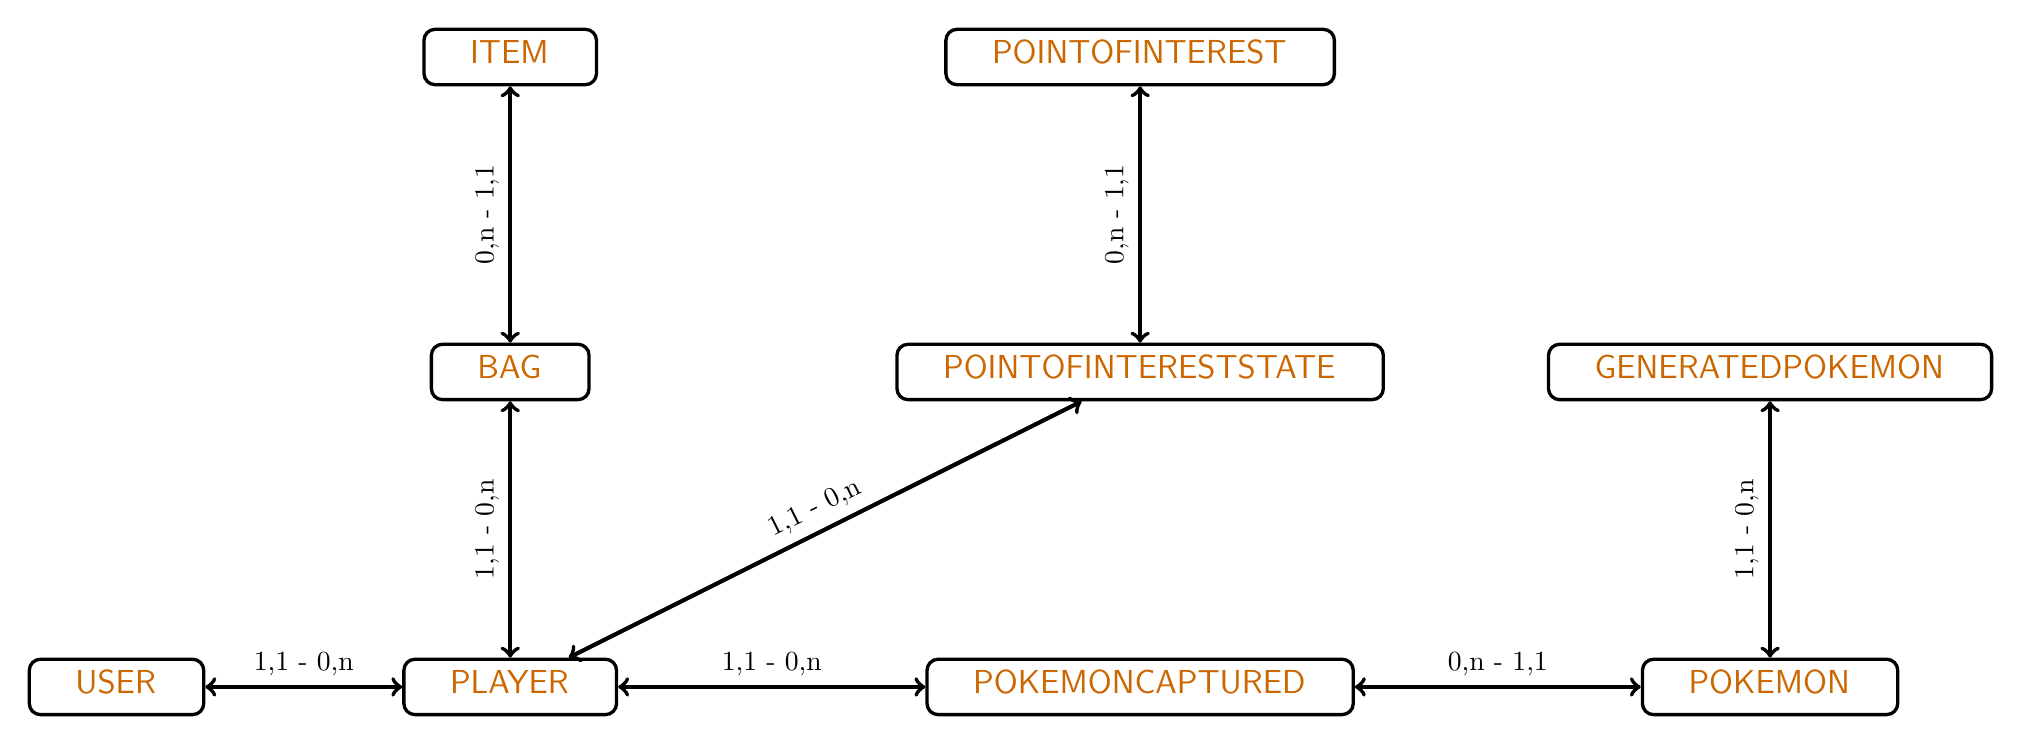
\begin{tikzpicture}

  \node[class] (USER) {
    \newtable{\type{USER}}{}
  };

  \node[class] (PLAYER) [right of=USER, node distance = 5cm] {
    \newtable{\type{PLAYER}}{}
  };

  \node[class] (POKCAPT) [right of=PLAYER, node distance = 8cm] {
    \newtable{\type{POKEMONCAPTURED}}{}
  };

  \node[class] (POKEMON) [right of=POKCAPT, node distance = 8cm] {
    \newtable{\type{POKEMON}}{}
  };

  \node[class] (GENPOKEMON) [above of=POKEMON, node distance = 4cm] {
    \newtable{\type{GENERATEDPOKEMON}}{}
  };

  \node[class] (BAG) [above of=PLAYER, node distance = 4cm] {
    \newtable{\type{BAG}}{}
  };

  \node[class] (ITEM) [above of=BAG, node distance = 4cm] {
    \newtable{\type{ITEM}}{}
  };

  \node[class] (POISTATE) [above of=PLAYER, node distance = 4cm, xshift=8cm] {
    \newtable{\type{POINTOFINTERESTSTATE}}{}
  };

  \node[class] (POI) [above of=POISTATE, node distance = 4cm] {
    \newtable{\type{POINTOFINTEREST}}{}
  };

  \path
  (USER)   edge [<->, line width=1.5pt, above] node {1,1 - 0,n} (PLAYER)
  (PLAYER) edge [<->, line width=1.5pt, above] node {1,1 - 0,n} (POKCAPT)
  (POKCAPT) edge [<->, line width=1.5pt, above] node {0,n - 1,1} (POKEMON)
  (POKEMON) edge [<->, line width=1.5pt, sloped, anchor=center, above] node {1,1 - 0,n} (GENPOKEMON)
  (PLAYER) edge [<->, line width=1.5pt, sloped, anchor=center, above] node {1,1 - 0,n} (BAG)
  (BAG) edge [<->, line width=1.5pt, sloped, anchor=center, above] node {0,n - 1,1} (ITEM)
  (PLAYER) edge [<->, line width=1.5pt, sloped, anchor=center, above] node {1,1 - 0,n} (POISTATE)
  (POISTATE) edge [<->, line width=1.5pt, sloped, anchor=center, above] node {0,n - 1,1} (POI)
  ;

\end{tikzpicture}

  \caption{Relational Model}
  \label{RELMODEL}
\end{sidewaysfigure}

\section{Extensions}


\end{document}

%%% Local Variables:
%%% mode: latex
%%% TeX-master: t
%%% End:
